% DO NOT COMPILE THIS FILE DIRECTLY!
% This is included by the the driver file (FlipBeamerTemplate.tex).

%{ %% This is a total kludge for a fancy title page background
%\setbeamertemplate{sidebar right}
 {\setbeamertemplate{sidebar right}{\llap{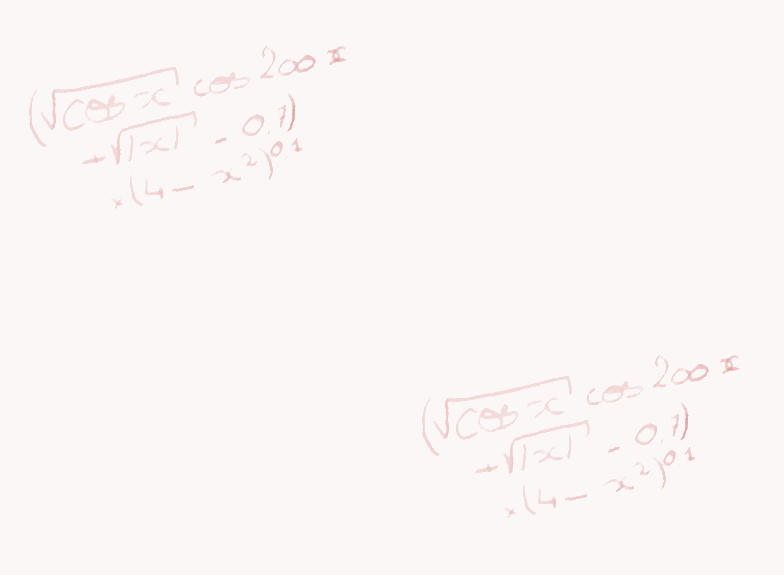
\includegraphics[width=\paperwidth,height=\paperheight]{BG_upper}}}
\begin{frame}[c]%{\phantom{title page}} 
% The \phantom{title page} is a kludge to get the red bar on top
% \titlepage
\begin{center}
	% \includegraphics[width=7cm]{WarpedPenguinsReturn}
%\vspace*{-2cm}
	\begin{tikzpicture}%[show background grid] %% Use grid for positioning, then turn off
		\node[inner sep=10pt,anchor =north west] (title) 
			{ \includegraphics[width=7cm]{\titleimage} };
			 \node (title) at (0.5,-2.5) {};
	\end{tikzpicture}
	\quad

	% \includegraphics[width=7cm]{\titleimage} 
	%\vspace*{1cm}
	\tiny{Céline Caldini-Queiros, Bruno Després, Lise-Marie Imbert-Gérard, Maryna Kachanovska\\ (with Olivier Lafitte and Remi Sart)}
	\vspace{.5em}
	
	\footnotesize\textcolor{brunfonce}{08.04.2014}
%	\texttt{[arXiv:1234.5678]}
	\vspace{1cm}
%	

\end{center}
\end{frame}}
\begin{frame}{Physical context and model}
 \begin{minipage}{0.45\linewidth}
 \begin{figure}
       		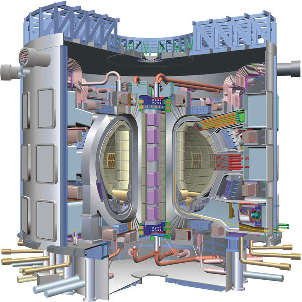
\includegraphics[scale = 0.7]{./images/ITER_cut}
       	\caption{ITER}
     	 \end{figure} 
\end{minipage}
\hfill
\begin{minipage}{0.45\linewidth}
 \begin{figure}
       		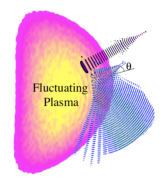
\includegraphics[scale = 1.2]{./images/antenne}
       		\caption{waves}
     	 \end{figure} 
\end{minipage}
\begin{block}{Equations : Maxwell-Newton}
\[
\begin{cases}
&-\frac{1}{c^2}\partial_t E + \nabla \wedge B = \mu_0 J \hspace{3cm} J = e N_e u_e\\
&\partial_t B + \nabla \wedge E  = 0	\\
&m_e \partial_t u_e  =  -e(E + u_e \wedge B_0 ) - m_e \nu u_e
\end{cases}
\]
\end{block}


\end{frame}
\begin{frame}{Some references on numerical simulation}
\begin{itemize}
\item Décomposition de domaines pour la simulation "full wave" dans un plasma froid, T. Hattori (thesis) \\ 
\item Analyse mathématique et numérique de problèmes d’ondes apparaissant dans les plasmas
magnétiques, L.-M. Imbert-Gérard (thesis)\\ 
\item Hybrid resonance of Maxwell's equations in slab geometry, B.Després, L.M. Imbert-Gérard and R. Weder, in JMPA\\ 
\item  Stable coupling of the Yee scheme with a linear current model, F. Da Silva, M. Campos-Pinto, B. Després, S. Heuraux, HAL preprint 2014. \\ 
\item Full-wave modeling of the O-X mode conversion in the Pegasus Toroidal Experiment, A. Kohn, J. Jacquot, M.W. Bongard, S. Gallian, E.T. Hinson and F.A. Volpe, arXiv:1104.0743 [physics.plasm-ph](2011).
\end{itemize}
\end{frame}
\begin{frame}{Frequency domain study}
In 1D :  $\partial_y = i \theta$. Unknowns : $\ubf =(E_1,E_2) = (E_x,E_y)$


\alert{Variational formulation :}
\[
\begin{array}{l}
\displaystyle \int_{-L}^H (E_2' -i\theta E_1)\overline{(\tilde E_2' -i \theta \tilde E_1)} - \int_{-L}^H (\eps_0 +i\nu Id) \E \cdot \overline{\tilde \E}
\\ \displaystyle  - i \sqrt{\alpha(-L)} E_2 (-L) \tilde E_2 (-L) = -g_{inc} (-L) \overline{( \tilde E_2(-L) )} 
\end{array}
\]
\[
a(\ubf,\vbf) = a_1 (\ubf,\vbf) +i a_2(\ubf,\vbf)\  \text{ and } \  l(\vbf) = -g_{inc} (-L) \overline{(v_2(-L) )} 
\]
\[
\left\{\begin{array}{l}
a_1(\ubf,\vbf) = \int_{-L}^H (u_2' -i\theta u_1)\overline{(v_2' -i \theta v_1)} - \int_{-L}^H \eps_0 \ubf\cdot \overline{\vbf}, 
\\ a_2(\ubf,\vbf) = -\nu \int_{-L}^H  \ubf\cdot \overline{\vbf} -  \sqrt{\alpha(-L)} u_2 (-L) \overline{v_2 (-L)} , 
\end{array}\right.
\]
where $a_1= a_1^*$ and $a_2=a_2^*$ are hermitian.
\[
\ubf,\vbf \in V =  \{ (E_1,E_2) |\; E_1,E_2,E_2'  \in L^2\}
\]
\[
\|u\|_{V}^2 = \|E_1\|^2_{L^2} + \|E_2\|^2_{L^2} + \|E_2'\|_{L^2}
\]
\end{frame}
\begin{frame}{Frequency domain study}
\[
|a(\ubf,\ubf)| \geq \frac{1}{4} \sqrt{\frac{\nu}{\heps + \theta^2}}\|u_2'\|^2_{L^2} +  \frac{\nu}{4} \|\ubf\|_{L^2}^2,
\]

\vspace*{0.5cm}
\begin{block}{}
\begin{itemize}
\item The problem is well-posed (existence/uniqueness)
\item Passing to the limit $\nu \rightarrow 0^+$ is the limit absorption principle
\end{itemize}
\end{block}
\end{frame}

\begin{frame}{Simulation in frequency domain}
\ALERT{Matlab code, $P^1$ FEM}

For physically adapted coefficients $N_e$, $B_0$ it yields the hybrid resonance 

\ \\

 \begin{minipage}{0.45\linewidth}
\begin{figure}
	\begin{center}
       	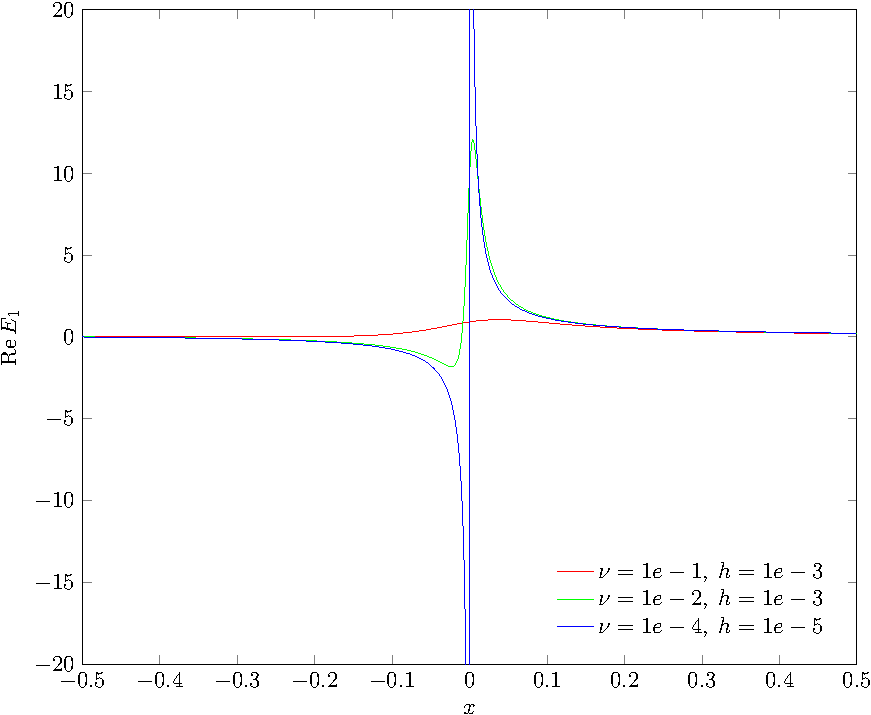
\includegraphics[width = 0.9\textwidth]{./images/picture2}
       	\caption{Convergence $E_x^\nu(x)$}
    \end{center}
\end{figure} 
\end{minipage}
\hfill
\begin{minipage}{0.45\linewidth}
	\begin{figure}
\begin{center}
       	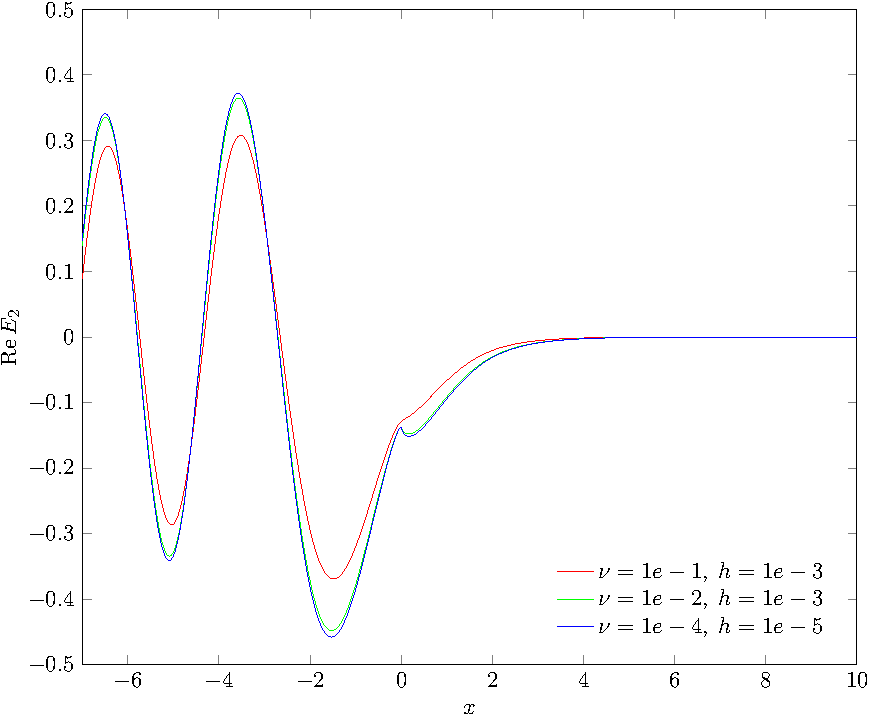
\includegraphics[width = 0.9\textwidth]{./images/pics3}
       	\caption{Convergence $E^\nu_y(x)$}
    \end{center}
\end{figure} 
\end{minipage}
\[
E_x^\nu \approx \frac{c}{x + i \nu}
\]

\end{frame}
\begin{frame}
\begin{figure}[ht]
\subfigure[\footnotesize{Convergence non sigular case}]{
    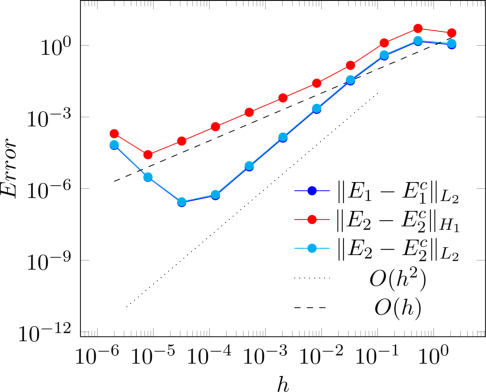
\includegraphics[width=0.38\textwidth]{./images/fig1}
  }
  \subfigure[\footnotesize{$E_x(x)$ error (singular case)}]{
    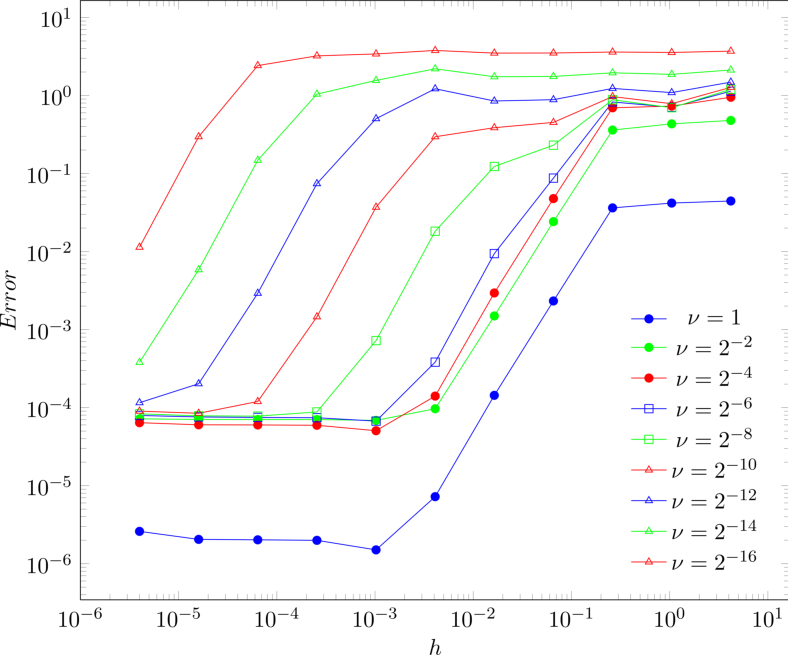
\includegraphics[width=0.38\textwidth]{./images/fig2}
  }
  
  \subfigure[$E_y(x)$ error (singular case)]{
    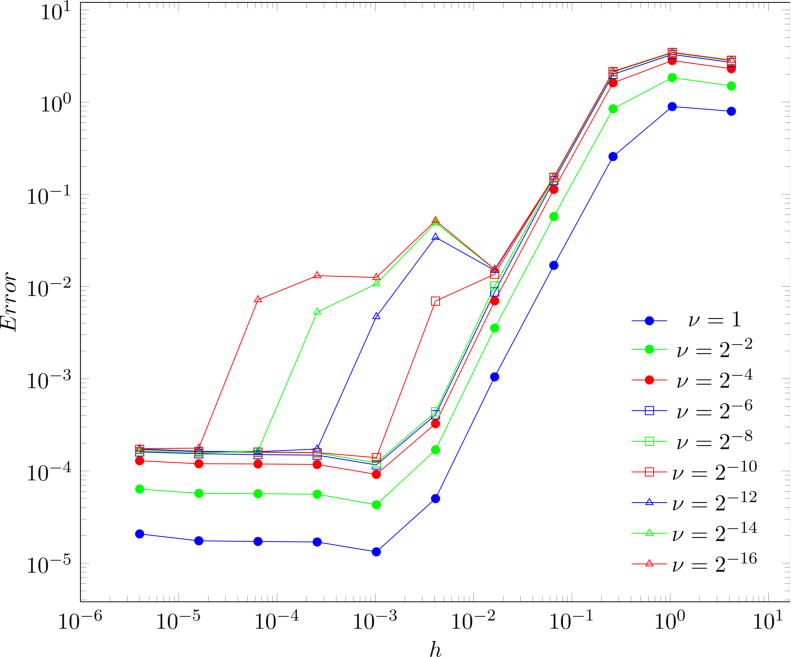
\includegraphics[width=0.38\textwidth]{./images/fig3}
  }
  \subfigure[$h_\veps$  vs $\nu$ (sing.)]{
    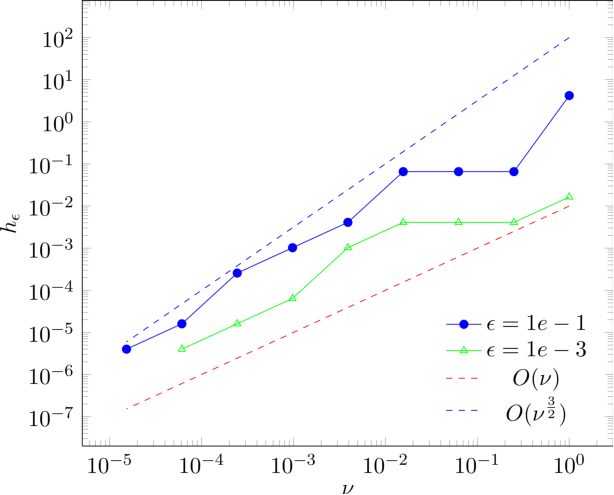
\includegraphics[width=0.38\textwidth]{./images/fig4}
  }
  
\end{figure}
\end{frame}

\begin{frame}{Time dependent problem}
Harmonic forcing on the boundary : recover the limiting amplitude principle\footnote{C. Morawetz, CPAM, 1962} at the limit $t\rightarrow \infty$ 
\[
\begin{cases}
- \veps_0 \partial_t E_x = e N_e u_x \\
- \veps_0 \partial_t E_y - \partial_x E_y =  e N_e u_y \\
\partial_t H_z + \partial_x E_y = 0 \\
m_e \partial_t u_x = e (E_x + u_y B_0) - \nu m_e u_x \\
m_e \partial_t u_y = e (E_x - u_x B_0) - \nu m_e u_y
\end{cases}
\]

\alert{Finite difference, 1D energy conservative leap-frog scheme\footnote{ Stable coupling of the Yee scheme with a linear current model, F. Da Silva, M. Campos-Pinto, B. Després, S. Heuraux, HAL preprint 2014}}

 \begin{center} \href{run:test.mp4}{\Alert{$\diamondsuit$}} \end{center}


\end{frame}
 {\setbeamertemplate{sidebar right}{\llap{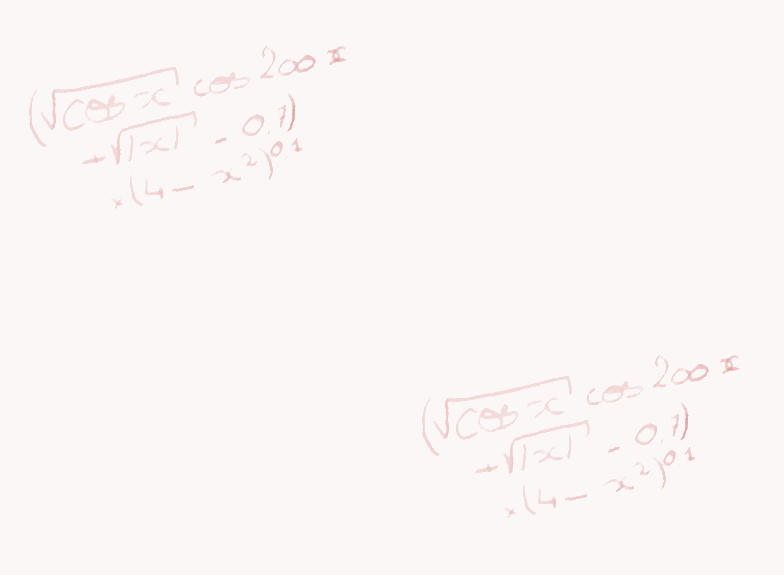
\includegraphics[width=\paperwidth,height=\paperheight]{BG_upper}}}
\begin{frame}
\begin{center}
\textcolor{lightred}{\scalebox{2}{Thank you for your attention !}}
\end{center}
\end{frame}}

